\documentclass[
	% -- opções da classe memoir --
	article,			% indica que é um artigo acadêmico
	12pt,				% tamanho da fonte
	oneside,			% para impressão apenas no recto. Oposto a twoside
	a4paper,			% tamanho do papel. 
	% -- opções da classe abntex2 --
	%chapter=TITLE,		% títulos de capítulos convertidos em letras maiúsculas
	%section=TITLE,		% títulos de seções convertidos em letras maiúsculas
	%subsection=TITLE,	% títulos de subseções convertidos em letras maiúsculas
	%subsubsection=TITLE % títulos de subsubseções convertidos em letras maiúsculas
	% -- opções do pacote babel --
	english,			% idioma adicional para hifenização
	brazil,				% o último idioma é o principal do documento
	sumario=tradicional
	]{abntex2}


% ---
% PACOTES
% ---

% ---
% Pacotes fundamentais 
% ---
\usepackage{babel}
\usepackage{lmodern}			% Usa a fonte Latin Modern
\usepackage[T1]{fontenc}		% Selecao de codigos de fonte.
\usepackage[utf8]{inputenc}		% Codificacao do documento (conversão automática dos acentos)
\usepackage{indentfirst}		% Indenta o primeiro parágrafo de cada seção.
\usepackage{nomencl} 			% Lista de simbolos
\usepackage{color}				% Controle das cores
\usepackage{graphicx}			% Inclusão de gráficos
\usepackage{microtype} 			% para melhorias de justificação
%\usepackage{uarial}			% Utilização da fonte Arial 
%\renewcommand{\familydefault}{\sffamily}% Causa crash no doc
%\usepackage[scaled]{helvet}		% Utilização da fonte Helvet 
%\renewcommand*\familydefault{\sfdefault} % O sumário deixa de ser feito
% ---
		
% ---
% Pacotes adicionais, usados apenas no âmbito do Modelo Canônico do abnteX2
% ---
\usepackage{lipsum}				% para geração de dummy text
% ---
		
% ---
% Pacotes de citações
% ---
\usepackage[brazilian,hyperpageref]{backref}	 % Paginas com as citações na bibl
\usepackage[alf]{abntex2cite}	% Citações padrão ABNT
% ---

% ---
% Configurações do pacote backref
% Usado sem a opção hyperpageref de backref
\renewcommand{\backrefpagesname}{Citado na(s) página(s):~}
% Texto padrão antes do número das páginas
\renewcommand{\backref}{}
% Define os textos da citação
\renewcommand*{\backrefalt}[4]{
	\ifcase #1 %
		Nenhuma citação no texto.%
	\or
		Citado na página #2.%
	\else
		Citado #1 vezes nas páginas #2.%
	\fi}%
% ---
% ---
% Informações de dados para CAPA e FOLHA DE ROSTO
% ---
\titulo{Manual do Software MadeOeste}
\autor{Otávio A. de Almeida \\ Cauê R. Sampaio \\ Ranan Augusto}
\local{Sorocaba}
\data{2018, v-1.0.2}
% ---
% ---
% Configurações de aparência do PDF final

% alterando o aspecto da cor azul
\definecolor{blue}{RGB}{41,5,195}

% informações do PDF
\makeatletter
\hypersetup{
	%pagebackref=true,
	pdftitle={\@title}, 
	pdfauthor={\@author},
	pdfsubject={Manual do Software MadeOeste},
	pdfcreator={LaTeX with abnTeX2},
	pdfkeywords={Manual}{MadeOeste}{TCC}{Fernendo Prestes}{Informática}, 
	colorlinks=true,       		% false: boxed links; true: colored links
	linkcolor=black,          	% color of internal links
	citecolor=blue,        		% color of links to bibliography
	filecolor=magenta,      		% color of file links
	urlcolor=blue,
	bookmarksdepth=4
}
\makeatother
% --- 
% ---
% compila o indice
% ---
\makeindex
% ---

% ---
% Altera as margens padrões
% ---
\setlrmarginsandblock{3cm}{2cm}{*}
\setulmarginsandblock{3cm}{2cm}{*}
\checkandfixthelayout
% ---

% --- 
% Espaçamentos entre linhas e parágrafos 
% --- 

% O tamanho do parágrafo é dado por:
\setlength{\parindent}{1.5cm}
% Controle do espaçamento entre um parágrafo e outro:
\setlength{\parskip}{0.2cm}  % tente também \onelineskip

% Espaçamento simples
\SingleSpacing

% --- DOCUMENT --- %
\begin{document}
	% --- Settings -- %
	% Seleciona o idioma do documento (conforme pacotes do babel)
	%\selectlanguage{english}
	\selectlanguage{brazil}	
	% Retira espaço extra obsoleto entre as frases.
	\frenchspacing
	
	% --- Folha de Rosto --- %
	\begin{folhaderosto}
		\centering
		\maketitle
		\vfill
		{Sorocaba\\2018}
	\end{folhaderosto}
	
	% --- Sumário --- %
	\newpage
	\tableofcontents
	
	% --- Menu Principal --- %
	\newpage
	\section{Menu Principal}
		\begin{figure}[!htb]
			\centering
			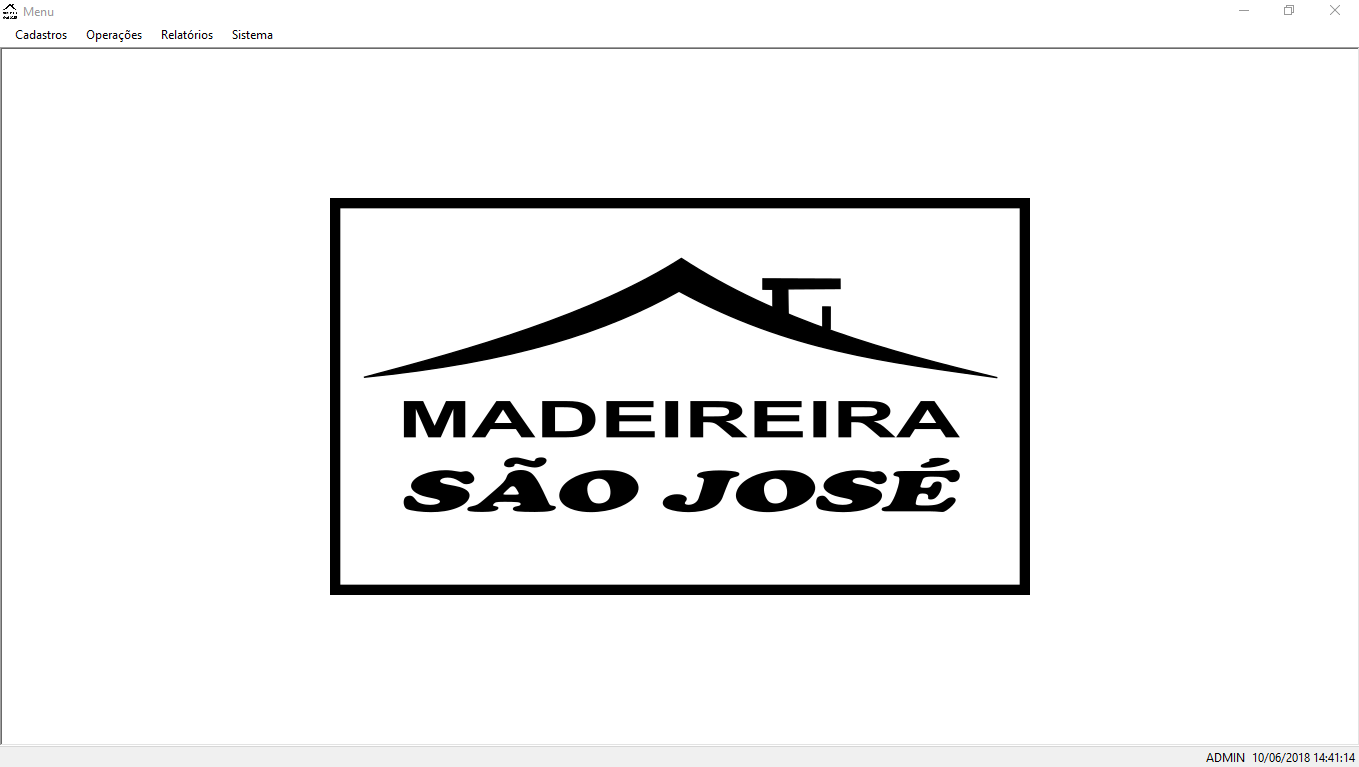
\includegraphics[scale=0.7]{./Figuras/FrmMenu.png}
			\caption{Formulário do Menu Principal}
		\end{figure}
		\subsection{Objetivo}
		O Menu do Software é o ponto de acesso para todos os demais formulários e relatórios.
		\subsection{Funcionalidades}
			\begin{itemize}
				\item Acessar todos os formulários
				\item Acessar todos os relatórios
				\item Informar a hora e o usuário logado
		    \end{itemize}
		\subsection{Componentes}
		Na parte superior, há, da esquerda para a direita, duas abas, a aba de cadastros e a aba de relatórios.
		Na parte inferior da tela, há um menu de status que apresenta a data e hora atuais do sistema e o usuário que está logado no sistema.
		\subsubsection{Aba de Cadastros}
		Quando a aba de cadastros é pressionada, todos os índices dos formulários referentes ao sistema são exibidos, clicando em um desses índices, o formulário correspondente é aberto, caso já esteja aberto, o formulário aberto é exposto à frente dos demais.
		\subsubsection{Aba de Relatórios}
		Quando a aba de relatórios é pressionada, todos os índices dos relatórios referentes ao sistema são exibidos, clicando em um desses índices, o relatório correspondente é aberto, caso já esteja aberto, o formulário aberto é fechado e um novo é aberto para o caso de atualização de informações.
	\newpage
	\section{Formulário de Clientes}
		\begin{figure}[!htb]
			\centering
			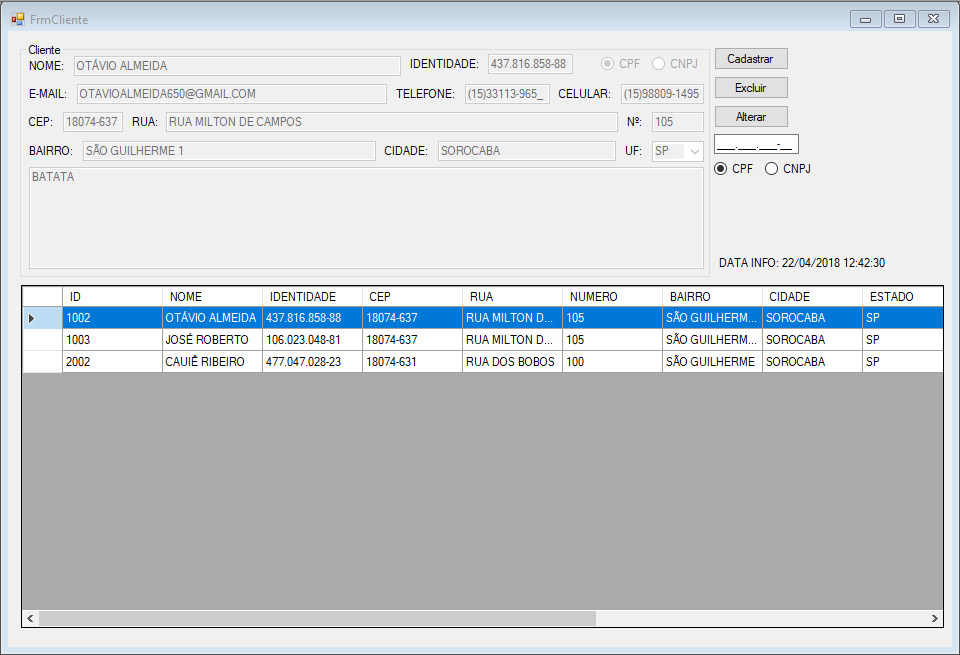
\includegraphics[scale=0.6]{./Figuras/FrmCliente.png}
			\caption{Formulário de Clientes}
		\end{figure}	
		\subsection{Objetivo}
		O formulário de clientes tem o objetivo de cadastrar novos clientes no sistema, alterar e excluir os existentes e pesquisar os clientes cadastrados de acordo com a sua identidade.
		\subsection{Funcionalidades}
			\begin{itemize}
				\item Cadastrar um novo cliente
				\item Excluir um cliente pela sua identidade
				\item Atualizar as informações de um cliente
				\item Acessar informações dos clientes cadastrados
			\end{itemize}	
		\subsection{Componentes}
			\subsubsection{Região de dados}
			O formulário de clientes terá uma região de dados, que ocupa a região superior esquerda da tela, destinada a inserção dados de um cliente caso a operação seja de cadastro ou alteração, ou de exibição de dados específicos caso um registro seja selecionado na tabela.
			Os componentes dessa região são:
				\begin{itemize}\itemsep1.5pt
					\item Nome do cliente
					\item A identidade do cliente, podendo ser tanto o CPF quanto o CNPJ.
					\item O e-mail do cliente
					\item O telefone principal do cliente
					\item O telefone celular do cliente
					\item O CEP do cliente
					\item A rua do cliente
					\item O número da localidade do cliente
					\item O bairro do cliente
					\item A cidade do cliente
					\item A unidade federativa do cliente
					\item As observações sobre o cliente
				\end{itemize}
			\subsubsection{Região de operações e miscelânea}
			A região superior direita é destinada aos botões de operação, o campo de filtro por identidade e a data da informação que está selecionada na tabela.
			\subsubsection{Região da Tabela}
			A parte inferior é uma tabela que mostra todos os clientes registrados no sistema caso não haja filtro, senão ela mostra todos os clientes registrados que coincidem com o filtro.
	\newpage
	\section{Formulário de Fornecedores}
		\begin{figure}[!htb]
			\centering
			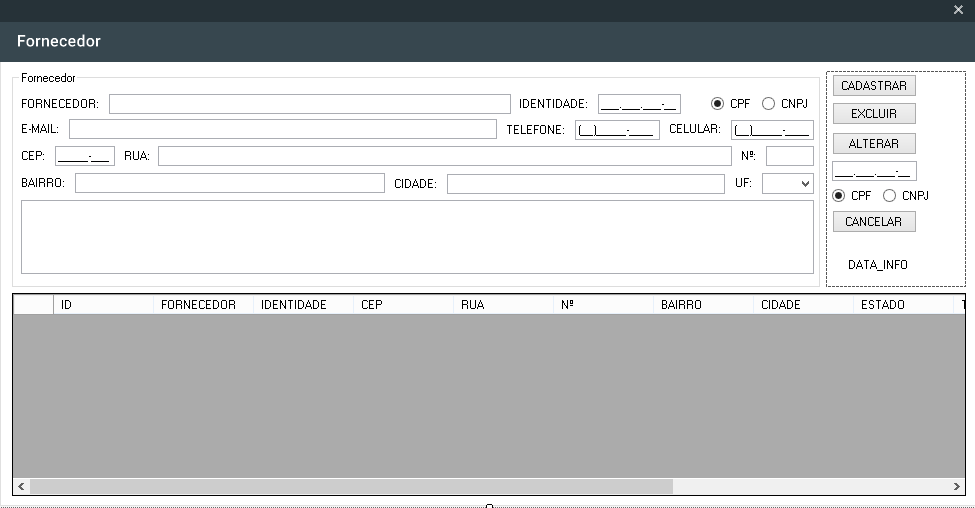
\includegraphics[scale=0.6]{./Figuras/FrmFornecedor.png}
			\caption{Formulário de Fornecedores}
		\end{figure}
		\subsection{Objetivo}
		O formulário de fornecedores tem o objetivo de cadastrar novos fornecedores no sistema, alterar e excluir os existentes e pesquisar os fornecedores cadastrados de acordo com a sua identidade.
		\subsection{Funcionalidades}
			\begin{itemize}
			\item Cadastrar um novo fornecedor
			\item Excluir um fornecedor pela sua identidade
			\item Atualizar as informações de um fornecedor
			\item Acessar informações dos fornecedores cadastrados
			\end{itemize}
		\subsection{Componentes}
			\subsubsection{Região de dados}
			O formulário de fornecedores terá uma região de dados, que ocupa a região superior esquerda da tela, destinada a inserção dados de um fornecedor caso a operação seja de cadastro ou alteração, ou de exibição de dados específicos caso um registro seja selecionado na tabela.
			Os componentes dessa região são:
			\begin{itemize}\itemsep1.5pt
				\item Nome do fornecedor
				\item A identidade do fornecedor, podendo ser tanto o CPF quanto o CNPJ.
				\item O e-mail do fornecedor
				\item O telefone principal do fornecedor
				\item O telefone celular do fornecedor
				\item O CEP do fornecedor
				\item A rua do fornecedor
				\item O número da localidade do fornecedor
				\item O bairro do fornecedor
				\item A cidade do fornecedor
				\item A unidade federativa do fornecedor
				\item As observações sobre o fornecedor
			\end{itemize}	
			\subsubsection{Região de operações e miscelânea}
			A região superior direita é destinada aos botões de operação, o campo de filtro por identidade e a data da informação que está selecionada na tabela.
			\subsubsection{Região da Tabela}
			A parte inferior é uma tabela que mostra todos os fornecedores registrados no sistema caso não haja filtro, senão ela mostra todos os fornecedores registrados que coincidem com o filtro.
	\newpage
	\section{Formulário de Vendas}
		\begin{figure}[!htb]
			\centering
			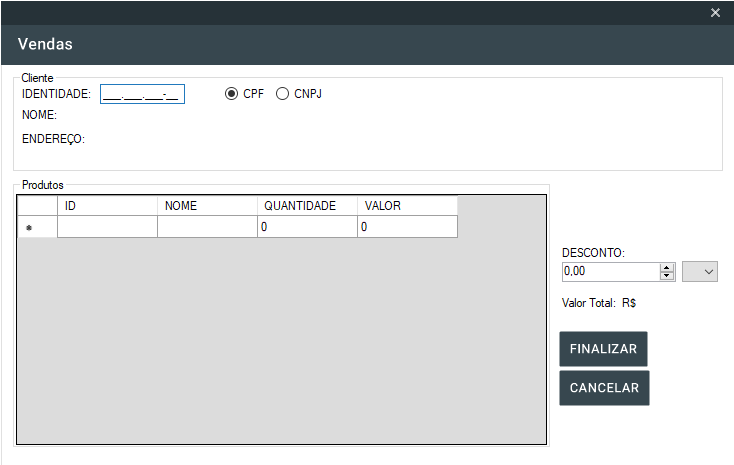
\includegraphics[scale=0.7]{./Figuras/FrmVenda.png}
			\caption{Formulário de Venda}
		\end{figure}
		\subsection{Objetivo}
		O formulário de vendas tem como objetivo fazer o registro das vendas que a madeireira recebe, além de atualizar o estoque das madeiras disponíveis.  
		\subsection{Funcionalidades}
			\begin{itemize}
				\item Cadastrar uma nova venda
				\item Adicionar e remover produtos de uma venda antes dela ser concluída ou cancelada
			\end{itemize}
		\subsection{Componentes}
			\subsubsection{Dados do Cliente}
			Esta região está destinado ao seleção do cliente, informando a identidade no campo de identidade, irá aparecer embaixo o nome e o endereço do cliente.
			\subsubsection{Produtos}
			Essa região é destinada a apresentação dos produtos que estão sendo inseridos junto com esta venda.
			\subsubsection{Operações de produtos}
			Esta região é compreendida por dois botões de adicionar e remover produtos.
			
			O botão adicionar chamará o formulário de inserção de produto em operações para fazer um novo registro de um produto para este fornecimento.
			
			O botão remover irá remover o produto selecionado na tabela de produtos do registro de fornecimento.
			\subsubsection{Operações de Venda}
			Esta região é compreendida por dois botões de concluir e cancelar venda.
			
			O botão concluir irá encerrar a venda e fará o registro no Banco de Dados.
			
			O botão cancelar irá encerrar a venda e não fará o registro no Banco de Dados.
	\newpage
	\section{Formulário de Fornecimentos}
		\begin{figure}[!htb]
			\centering
			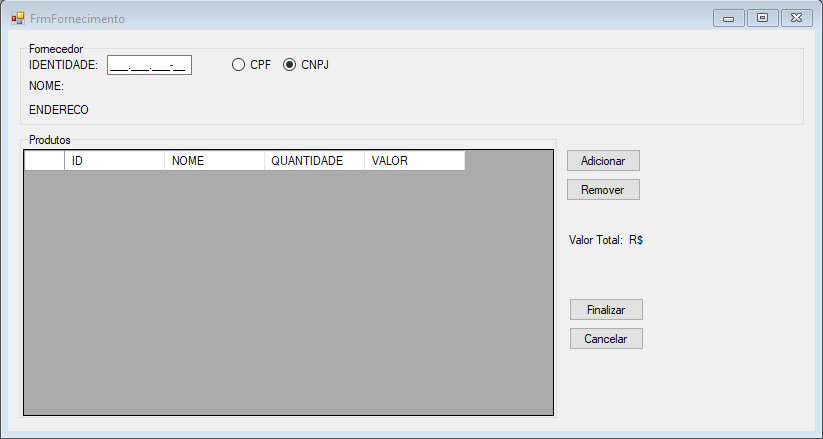
\includegraphics[scale=0.7]{./Figuras/FrmFornecimento.png}
			\caption{Formulário de Fornecimentos}
		\end{figure}
		\subsection{Objetivo}
		O formulário de fornecimento tem como objetivo fazer o registro dos fornecimentos que a madeireira recebe, além de atualizar o estoque das madeiras disponíveis.  
		\subsection{Funcionalidades}
			\begin{itemize}
			\item Cadastrar um novo fornecimento
			\item Adicionar e remover produtos de um fornecimento antes de ele ser concluído ou antes de ele ser cancelado 
			\end{itemize}
		\subsection{Componentes}
			\subsubsection{Dados do Fornecedor}
			Esta região está destinado ao seleção do fornecedor, informando a identidade no campo de identidade ou buscando atráves da lista de fornecedores, irá aparecer embaixo o nome e o endereço do fornecedor.
			\subsubsection{Produtos}
			Essa região é destinada a apresentação dos produtos que estão sendo inseridos junto com este fornecimento
			\subsubsection{Operações de produtos}
			Esta região é compreendido por dois botões de adicionar e remover produtos.
			
			O botão adicionar chamará o formulário de inserção de produto em operações para fazer um novo registro de um produto para este fornecimento.
			
			O botão remover irá remover o produto selecionado na tabela de produtos do registro de fornecimento.
	
	\newpage
	\section{Formulário de Funcionários}
		\begin{figure}[!htb]
			\centering
			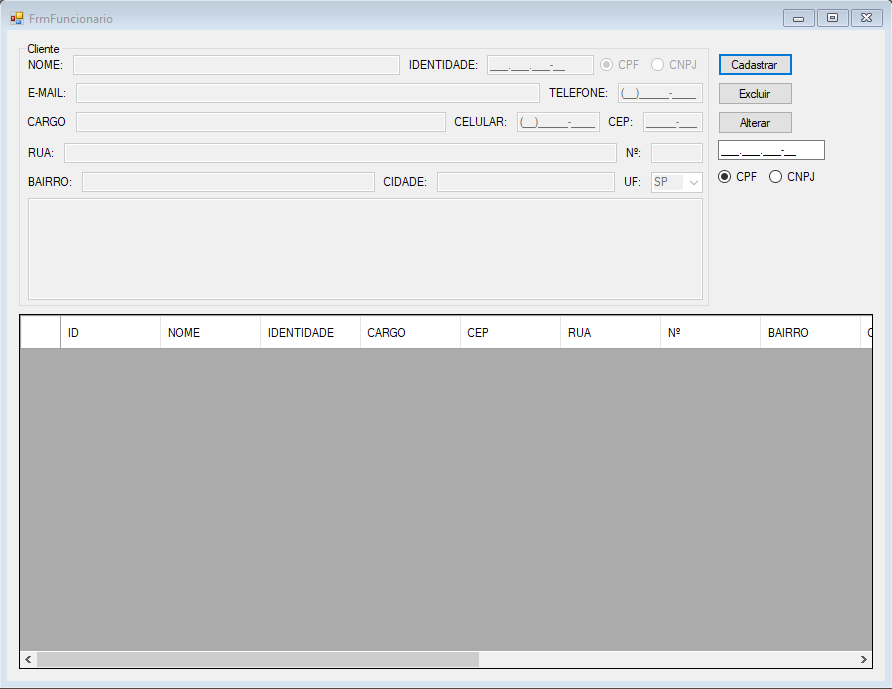
\includegraphics[scale=0.6]{./Figuras/FrmFuncionario.png}
			\caption{Formulário de Funcionários}
		\end{figure}
		\subsection{Objetivo}
		O formulário de funcionários tem o objetivo de cadastrar novos funcionário no sistema, alterar e excluir os existentes e pesquisar os funcionários cadastrados de acordo com a sua identidade.
		\subsection{Funcionalidades}
			\begin{itemize}
				\item Cadastrar um novo funcionário
				\item Excluir um funcionário pela sua identidade
				\item Atualizar as informações de um funcionário
				\item Acessar informações dos funcionários cadastrados
			\end{itemize}
		\subsection{Componentes}
			\subsubsection{Região de dados}
			O formulário de funcionários terá uma região de dados, que ocupa a região superior esquerda da tela, destinada a inserção dados de um funcionário caso a operação seja de cadastro ou alteração, ou de exibição de dados específicos caso um registro seja selecionado na tabela.
			
			Os componentes dessa região são:
			\begin{itemize}\itemsep1.5pt
				\item Nome do funcionário
				\item Cargo do funcionário
				\item A identidade do funcionário, podendo ser tanto o CPF quanto o CNPJ.
				\item O e-mail do funcionário
				\item O telefone principal do funcionário
				\item O telefone celular do funcionário
				\item O CEP do funcionário
				\item A rua do funcionário
				\item O número da localidade do funcionário
				\item O bairro do funcionário
				\item A cidade do funcionário
				\item A unidade federativa do funcionário
				\item As observações sobre o funcionário
			\end{itemize}	
			\subsubsection{Região de operações e miscelânea}
			A região superior direita é destinada aos botões de operação, o campo de filtro por identidade e a data da informação que está selecionada na tabela.
			\subsubsection{Região da Tabela}
			A parte inferior é uma tabela que mostra todos os funcionários registrados no sistema caso não haja filtro, senão ela mostra todos os funcionários registrados que coincidem com o filtro.
	\newpage
	\section{Formulário de Produtos}
		\begin{figure}[!htb]
			\centering
			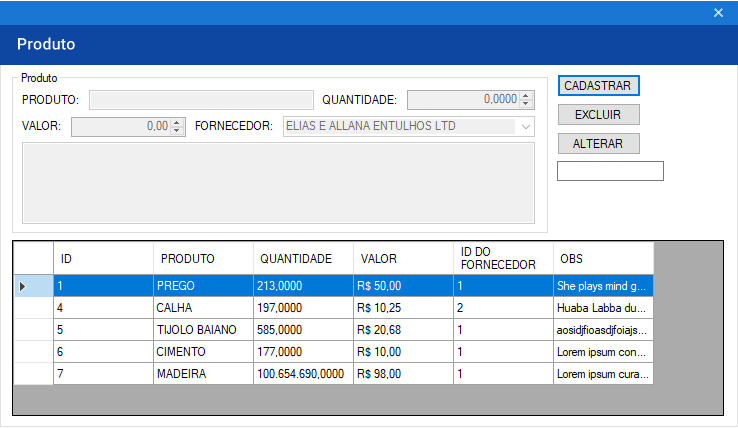
\includegraphics[scale=0.7]{./Figuras/FrmProduto.png}
			\caption{Formulário de Produtos}
		\end{figure}
		\subsection{Objetivo}
		O formulário de produtos tem o objetivo de cadastrar novos produtos no sistema, alterar e excluir os existentes e pesquisar os produtos cadastrados de acordo com a sua código.
		\subsection{Funcionalidades}
			\begin{itemize}
				\item Cadastrar um novo produto
				\item Excluir um produto pelo seu código
				\item Atualizar as informações de um produto
				\item Acessar informações dos produtos cadastrados
			\end{itemize}
		\subsection{Componentes}
			\subsubsection{Região de dados}
			O formulário de produtos terá uma região de dados, que ocupa a região superior esquerda da tela, destinada a inserção dados de um produto caso a operação seja de cadastro ou alteração, ou de exibição de dados específicos caso um registro seja selecionado na tabela.
			
			Os componentes dessa região são:
			\begin{itemize}\itemsep1.5pt
				\item Nome do produto
				\item A quantidade do produto
				\item O valor do produto
				\item O fornecedor do produto
				\item As observações sobre o produto
			\end{itemize}	
			\subsubsection{Região de operações e miscelânea}
			A região superior direita é destinada aos botões de operação, o campo de filtro por código e a data da informação que está selecionada na tabela.
			\subsubsection{Região da Tabela}
			A parte inferior é uma tabela que mostra todos os produtos registrados no sistema caso não haja filtro, senão ela mostra todos os produtos registrados que coincidem com o filtro.
\newpage
	\section{Formulário de I.P.O (Inserção de Produto em Operações)}
		\begin{figure}[!htb]
			\centering
			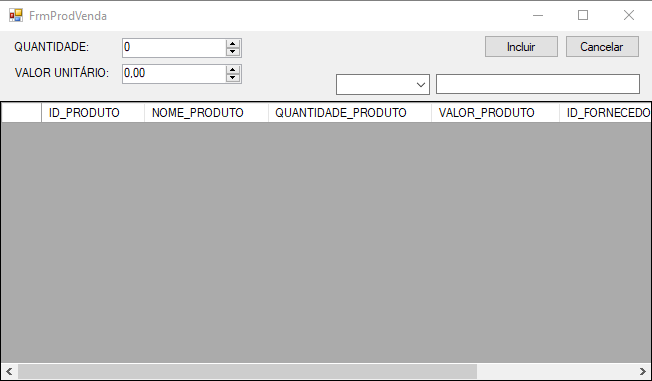
\includegraphics[scale=0.9]{./Figuras/FrmProdVenda.png}
			\caption{Formulário de Inserção de Produto em Operações}
		\end{figure}
		\subsection{Objetivo}
		O formulário de I.P.O tem o objetivo de cadastrar novos produtos em uma venda ou fornecimento.
		\subsection{Funcionalidades}
		\begin{itemize}
			\item Incluir um novo produto em uma venda ou fornecimento
			\item Acessar informações dos produtos cadastrados
		\end{itemize}
		\subsection{Componentes}
			\subsubsection{Região de dados}
			O formulário de I.P.O terá uma região de dados, que ocupa a região superior esquerda da tela, destinada a inserção dados de um produto para o fornecimento ou venda especificados. 
			
			Os componentes dessa região são:
			\begin{itemize}\itemsep1.5pt
				\item A quantidade do produto
				\item O valor do produto
			\end{itemize}	
			\subsubsection{Região de operações e miscelânea}
			A região superior direita é destinada aos botões de operação, o campo de filtro por código ou nome do produto.
			\subsubsection{Região da Tabela}
			A parte inferior é uma tabela que mostra todos os produtos registrados no sistema caso não haja filtro, senão ela mostra todos os produtos registrados que coincidem com o filtro.
			
			Essa região é importante porque o produto selecionado na tabela será repassado no formulário de venda ou fornecimento especificados.
	\newpage
	\section{Formulário de Usuários}
		\begin{figure}[!htb]
			\centering
			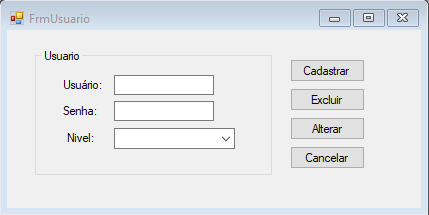
\includegraphics[scale=1.3]{./Figuras/FrmUsuario.png}
			\caption{Formulário de Usuários}
		\end{figure}
		\subsection{Objetivo}
		O formulário de usuário tem o objetivo de cadastrar novos usuários no sistema, alterar e excluir os existentes.
		\subsection{Funcionalidades}
			\begin{itemize}
				\item Incluir um novo usuário no sistema
				\item Alterar as informações de um usuário cadastrado
				\item Excluir um usuário cadastrado no sistema
			\end{itemize}
		\subsection{Componentes}		
			\subsubsection{Região de Dados}
			O formulário de usuários terá uma região de dados, que ocupa a região esquerda da tela, destinada a inserção dados de um usuário para o sistema.
			\subsubsection{Região de Operações}
			A região direita é destinada aos botões de operação.
	\newpage
	\section{Formulário de Login}
		\begin{figure}[!htb]
			\centering
			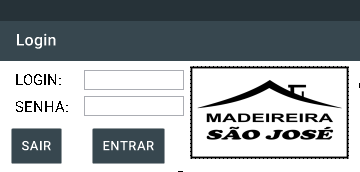
\includegraphics[scale=1.4]{./Figuras/FrmLogin.png}
			\caption{Formulário de Login}
		\end{figure}
		\subsection{Objetivo}
		O formulário de login tem como objetivo controlar o acesso ao sistema.
		
		O acesso só será permitido para usuário já cadastrados no sistema.
		\subsection{Funcionalidades}
		\begin{itemize}
			\item Obter acesso ao sistema por meio de um usuário e senha
		\end{itemize}
		\subsection{Componentes}
		Os componentes dessa região são:
		\begin{itemize}\itemsep1.5pt	
			\item Usuário: Campo destinado a entrada do nome do usuário
			\item Senha: Campo destinado a entrada da senha do usuário	
			\item Botão Entrar: Verifica os campos do usuário e senha e, se houver registro no sistema, garante acesso ao software	
			\item Botão Sair: Encerra a aplicação	
		\end{itemize}
\end{document}